%%%%%%%%%%%%%%%%%%%%%%%%%%%%%%%%%%%%%%%%%%%%%%%%%%%%%%%%%%%%%%%%%%%%%%%%%%%%
% AGUJournalTemplate.tex: this template file is for articles formatted with LaTeX
%
% This file includes commands and instructions
% given in the order necessary to produce a final output that will
% satisfy AGU requirements, including customized APA reference formatting.
%
% You may copy this file and give it your
% article name, and enter your text.
%
%
% Step 1: Set the \documentclass
%
%

%% To submit your paper:
\documentclass[draft]{agujournal2019}
\usepackage{url} %this package should fix any errors with URLs in refs.
\usepackage{lineno}
\usepackage[inline]{trackchanges} %for better track changes. finalnew option will compile document with changes incorporated.
\usepackage{soul}
%\linenumbers

%CMZ
\usepackage{natbib}
\usepackage{xcolor}
\usepackage{graphicx}
\newcommand{\degree}{$^{\circ}$}
\newcommand{\texttilde}{$\sim$}
\usepackage{tabularx}
\renewcommand\tabularxcolumn[1]{m{#1}}% for vertical centering text in X column

%%%%%%%
% As of 2018 we recommend use of the TrackChanges package to mark revisions.
% The trackchanges package adds five new LaTeX commands:
%
%  \note[editor]{The note}
%  \annote[editor]{Text to annotate}{The note}
%  \add[editor]{Text to add}
%  \remove[editor]{Text to remove}
%  \change[editor]{Text to remove}{Text to add}
%
% complete documentation is here: http://trackchanges.sourceforge.net/
%%%%%%%

\draftfalse

%% Enter journal name below.
%% Choose from this list of Journals:
%
% JGR: Atmospheres
% JGR: Biogeosciences
% JGR: Earth Surface
% JGR: Oceans
% JGR: Planets
% JGR: Solid Earth
% JGR: Space Physics
% Global Biogeochemical Cycles
% Geophysical Research Letters
% Paleoceanography and Paleoclimatology
% Radio Science
% Reviews of Geophysics
% Tectonics
% Space Weather
% Water Resources Research
% Geochemistry, Geophysics, Geosystems
% Journal of Advances in Modeling Earth Systems (JAMES)
% Earth's Future
% Earth and Space Science
% Geohealth
%
% ie, \journalname{Water Resources Research}

\journalname{Geophysical Research Letters}

\begin{document}

%% ------------------------------------------------------------------------ %%
%  Title
%
% (A title should be specific, informative, and brief. Use
% abbreviations only if they are defined in the abstract. Titles that
% start with general keywords then specific terms are optimized in
% searches)
%
%% ------------------------------------------------------------------------ %%



\title{Differences in algorithmic detection of rain-on-snow flood events across gridded data products}

%% ------------------------------------------------------------------------ %%
%
%  AUTHORS AND AFFILIATIONS!
%
%% ------------------------------------------------------------------------ %%

% Authors are individuals who have significantly contributed to the
% research and preparation of the article. Group authors are allowed, if
% each author in the group is separately identified in an appendix.)

% List authors by first name or initial followed by last name and
% separated by commas. Use \affil{} to number affiliations, and
% \thanks{} for author notes.
% Additional author notes should be indicated with \thanks{} (for
% example, for current addresses).

% Example: \authors{A. B. Author\affil{1}\thanks{Current address, Antartica}, B. C. Author\affil{2,3}, and D. E.
% Author\affil{3,4}\thanks{Also funded by Monsanto.}}

\authors{Colin M. Zarzycki\affil{1}, Benjamin D. Ascher\affil{1}\thanks{now at Colorado State University}, Alan M. Rhoades\affil{2}, and Rachel R. McCrary\affil{3}}


\affiliation{1}{Penn State}
\affiliation{2}{Climate and Ecosystem Sciences Division, Lawrence Berkeley National Laboratory, Berkeley, CA, USA}
\affiliation{3}{National Center for Atmospheric Research, Boulder, CO, USA}
% \affiliation{4}{Fourth Affiliation}

%% Corresponding Author:
% Corresponding author mailing address and e-mail address:

% (include name and email addresses of the corresponding author.  More
% than one corresponding author is allowed in this LaTeX file and for
% publication; but only one corresponding author is allowed in our
% editorial system.)

% Example: \correspondingauthor{First and Last Name}{email@address.edu}

\correspondingauthor{Colin M. Zarzycki}{cmz5202@psu.edu}

%% Keypoints, final entry on title page.

%  List up to three key points (at least one is required)
%  Key Points summarize the main points and conclusions of the article
%  Each must be 100 characters or less with no special characters or punctuation and must be complete sentences

% Example:
% \begin{keypoints}
% \item	List up to three key points (at least one is required)
% \item	Key Points summarize the main points and conclusions of the article
% \item	Each must be 100 characters or less with no special characters or punctuation and must be complete sentences
% \end{keypoints}

\begin{keypoints}
\item Rain-on-snow event detection algorithms can objectively isolate historical extremes in gridded climate data products at the basin-scale.
\item Large discrepancies in both mean climatology and event statistics exist in historical data products representing the same time period.
\item Finer temporal data and more frequent atmosphere-land surface coupling increase the number of flagged events.
\end{keypoints}

%% ------------------------------------------------------------------------ %%
%
%  ABSTRACT and PLAIN LANGUAGE SUMMARY
%
% A good Abstract will begin with a short description of the problem
% being addressed, briefly describe the new data or analyses, then
% briefly states the main conclusion(s) and how they are supported and
% uncertainties.

% The Plain Language Summary should be written for a broad audience,
% including journalists and the science-interested public, that will not have 
% a background in your field.
%
% A Plain Language Summary is required in GRL, JGR: Planets, JGR: Biogeosciences,
% JGR: Oceans, G-Cubed, Reviews of Geophysics, and JAMES.
% see http://sharingscience.agu.org/creating-plain-language-summary/)
%
%% ------------------------------------------------------------------------ %%

%% \begin{abstract} starts the second page
 
% CMZ, assuming 5 figures/tables, we have 3500 to work with!
 	
% The formula for PU = number of words/500 + number of figures + number of tables. Articles exceeding a certain amount of PUs incur excess page fees.
%
%Word count includes abstract, acknowledgements, text (and in-text citations), figure captions, table captions, and appendices. Equations count as one word no matter the size. Equations are not copyedited.
%
%Word count excludes title, author list and affiliations, key words, key points, plain language summary, table text, open research section, references, and supporting information. Supporting information is not copyedited.

\begin{abstract}
\color{blue} SAMPLE ABSTRACT FOR WORD COUNT! The northeastern United States is vulnerable to many impacts from snowfall-producing winter cyclones that are amplified by the proximity of population centers to storm tracks. Historically, climatic snowfall assessments have centered around seasonal means even though local impacts typically occur at scales of hours to days. To detect snowstorms at the event level, an objective algorithm is defined based on the Regional Snowfall Index. The metric collocates storm snowfall with population to produce statistics of snowstorms with societal impacts. When applied to the Community Earth System Model Large Ensemble (LENS), broad declines in snowstorm frequency are projected by the later 21st century. These decreases are primarily due to a warmer atmosphere less conducive to snowfall as the predominant precipitation type. However, reductions are less significant for major events, since more hostile thermodynamic environments are partially offset by increased precipitation associated with cyclones that dynamically drive high-impact snowstorms.
\end{abstract}

\section*{Plain Language Summary}
{\color{blue} Colin will write something here when submitting, not included in word count!}

%%% STUFF TO ADD
% Comment about how RoS is a compound extreme + cite Kai's paper
% Add what variables in E3SM were nudged + provide namelists in final repo.

%% ------------------------------------------------------------------------ %%
%
%  TEXT
%
%% ------------------------------------------------------------------------ %%

%%% Suggested section heads:
% \section{Introduction}
%
% The main text should start with an introduction. Except for short
% manuscripts (such as comments and replies), the text should be divided
% into sections, each with its own heading.

% Headings should be sentence fragments and do not begin with a
% lowercase letter or number. Examples of good headings are:

% \section{Materials and Methods}
% Here is text on Materials and Methods.
%
% \subsection{A descriptive heading about methods}
% More about Methods.
%
% \section{Data} (Or section title might be a descriptive heading about data)
%
% \section{Results} (Or section title might be a descriptive heading about the
% results)
%
% \section{Conclusions}


\section{Introduction}
%Text here ===>>>

While rain-on-snow (RoS) events have been studied over the past few decades in North America, research has overwhelmingly focused on mountainous regions \citep{singh1997hydrological,mccabe2007rain,musselman2018projected}. 
Correspondingly, there has been less focus in areas with more ephemeral snow cover, even though these discrete, extreme, and compound events are key drivers of `slow-rise' flooding -- flood events generally occurring more than six hours after the onset of the meteorological driver \citep{dougherty2021high} -- in the northeastern United States (US). 
Climatologically, RoS events in the northeastern US peak in late winter and spring \citep{ashley2008flood,villarini2010flood,dougherty2019climatology} and are a key driver of flooding in New England and Atlantic Canada \citet{collins2014annual}. 
\citet{wachowicz2020rain} found that the majority of RoS events occur in spring through the production of a pointwise climatology of RoS events in the eastern US using the dataset of \citet{dyer2006spatial}. \citet{grote2021synoptic} composited the synoptic meteorological fields of six recent RoS events in the mid-Atlantic region and found that flooding was driven by an inland-running extratropical cyclone that advected warm, moist air in the warm sector of the cyclone into the study region. 
Rapid snow ablation in regions with ephemeral snow has been shown to have a strong correlation with subsequent increases in basin streamflow. 
In the Susquehanna River Basin (SRB), \citet{suriano2020discharge} found that 75\% of snow ablation events (defined by a daily decrease in snow depth in above-freezing conditions) yielded increased river discharge three days later.

While climatological studies such as those described above are critically important, event-level analysis has become increasingly important when communicating climate risks \citep{shepherd2018storylines}. 
The most consequential non-tropical-cyclone flood in recent SRB history was a RoS flood that occurred in January 1996, causing substantial flooding that resulted in $\sim$\$1.5 billion in damages and 30 fatalities \citep{leathers1998severe}.
Significant events such as this one are frequently used by stakeholders as a point of reference for real-time forecasts and long-term planning \citep{george2019the}. 
Although these events are useful for planning purposes, quantifying extreme, compound, and discrete events is a complex challenge, particularly with gridded climate data products that are often developed for a myriad of purposes combined with a lack of observational reference datasets to quantify their fidelity. 
To extract information regarding compound hydrometeorological extreme events, such as RoS events, and their corresponding statistics, algorithmic techniques which objectively analyze datasets without manual intervention need to be devised.
Here, we demonstrate a technique for generating a RoS event database at the basin-scale for any arbitrary gridded dataset and intercompare key decision-relevant differences (e.g., flood magnitude) across four publicly available gridded climate data products. 


%We focus on the direct prediction of coupled surface processes (i.e., snow water equivalent and surface runoff) to minimize issues with statistical or dynamical downscaling and permit a like-to-like comparison between different datasets.

\section{Methods}

\subsection{Datasets}

We evaluate RoS events within three widely-used climate datasets and in one state-of-the-art Earth system model (ESM) nudged to reanalysis. All four products seek to reproduce observed conditions, although each uses a distinct methodology to do so. 
First, we investigate the dataset described in \citet{livneh2015spatially} (L15). 
L15 is a 1/16\degree{} hydrometeorological dataset covering most of North America. 
Meteorological data consists of daily precipitation, temperature, and wind speed \citep{henn2018an}. 
This data is then used to drive the Variable Infiltration Capacity (VIC, \citet{liang1994simple}) model to produce hydrometeorological outputs. 
Next, we investigate the 1/8\degree{} North American Land Data Assimilation System (NLDAS-VIC4.0.5)  described in \citet{xia2012continental1}. 
NLDAS is driven by offline atmospheric forcing derived from the North American Regional Reanalysis, with adjustments made based on observations such as from precipitation gauges. 
Of note, NLDAS uses a combination of daily precipitation observations and radar data to produce hourly estimates. 
While there are four NLDAS-2 land surface models (LSMs) that produce hydrologic output variables, we analyze only the NLDAS-VIC4.0.5 to be somewhat consistent with L15.
We also analyze a $\sim$0.5\degree{} global reanalysis (JRA-55, \citet{kobayashi2015jra55}), generated by running a prognostic ESM while assimilating observational data during integration. 
Global reanalyses serve as a bridge between in-situ observational data and free-running climate models. 
Finally, a $\sim$1\degree{} nudged version of the U.S. Department of Energy Energy Exascale Earth System Model (E3SM) model is analyzed. Assessing this dataset provides insight regarding the capability of ESMs used in climate assessments (e.g., the Coupled Model Intercomparison Project Phase 6 (CMIP6)) to capture observed hydrologic events.
%E3SM is analogous to the majority of climate models in CMIP6. 
To constrain the large-scale meteorology in E3SM to be more akin to observed conditions, the E3SM simulation is nudged using 6-hourly snapshots from the ERA5 reanalysis \citep{herbash2020era5}.
This nudging acts as a crude assimilation technique and is only applied in the free atmosphere, reproducing patterns of 500 hPa geopotential height and sea level pressure while allowing the model to simulate grid-scale processes relatively freely \citep{sun2019impact}. 
While E3SM is run on an unstructured cubed-sphere mesh, simulation output is regridded to a 1\degree{}x1\degree{} rectilinear grid.
%using higher-order methods \citep{hill2004architecture}. 

\subsection{Defining basin-scale events}

To identify RoS events, three variables are extracted over the SRB across all gridded climate datasets. 
These include precipitation (PRECIP), snow water equivalent (SWE), and surface water runoff (ROF). 
The 24-hour change in SWE from the previous day (dSWE) is calculated via a backward difference. 
All data is standardized to daily average values (00Z to 00Z) by temporally-averaging any sub-daily (e.g., hourly) data at each grid cell.
Grid cells that have at least 50\% of their area enclosed by the boundary of the SRB are kept, while those exterior to the SRB ($>$50\%) are set to missing values. 
The resulting domains for each product can be seen in Fig. \ref{fig:means}. A basin-wide time series is then constructed by spatially averaging the three fields for each day and smoothing the resulting time series using a moving average to reduce day-to-day noise in the derived variables. 
We choose a 5-day window based on synoptic timescales \citep{holton2004introduction}, although different windows didn't materially change any findings.

RoS days are defined algorithmically by flagging concurrent temporal windows of negative dSWE and positive ROF that both exceed pre-defined thresholds in the smoothed time series. 
We test two methods of thresholding; one uses fixed thresholds across all four datasets (FIXED) and the other defines dataset-specific thresholds by those exceeding 95\% of all daily values (RELATIVE). 
For fixed thresholds, we require an average dSWE of -1.4 mm/day and ROF of 1.4 mm/day based on a manual sensitivity analysis. To enforce a criterion that precipitation occurs during at least some portion of the event, we require an average PRECIP of 2 mm/day. 
To confirm all datasets adequately represent the same period, Pearson correlations of basin-wide statistics were statistically significant with a two-sided $t$-test between all permutations of daily timeseries (Table SX), confirming all datasets adequately represent the same period.

%Note that while the majority of the events are associated with PRECIP we do not include a specific criterion, but rather, leverage ROF as a proxy for surface flooding. 

\section{Results}

\subsection{Climatology}

The average November to April spatial climatologies of PRECIP, SWE, ROF, and dSWE are shown in Figure \ref{fig:means}. 
The higher resolution of L15 and NLDAS is evident from the added structure in the mean fields. 
Mean PRECIP (Fig. \ref{fig:means}a-d) is higher in JRA and E3SM when compared to the L15 and NLDAS. 
This may be due to factors such as atmospheric model biases or the inclusion of gauge data in L15 and NLDAS, although it has been shown that significant spread exists in historical gridded climate data products, even for more commonly observed variables such as PRECIP \citep{gutmann2012comparison,livneh2014filling,henn2018an}.
Both ROF (Figure \ref{fig:means}e-h) and SWE (Figure \ref{fig:means}i-l) climatologies differ between the data products. 
Notably, L15 produces mean ROF values that are less than half of the climatologies of each of the three other gridded climate data products. 
Conversely, NLDAS produces less SWE climatologically, $<$20\% of the SWE produced by L15 or E3SM and even less than the coarser JRA product. 
It is well-known that simulated ROF from different hydrologic models can be extremely variable, with regional differences between products reaching an order of magnitude in some cases \citep{gudmundsson2012comparing,sood2015global,beck2017global}. 
Previous work has also shown that SWE estimates can vary greatly across datasets \citep{lundquist2015high,Rhoades2018a}, particularly over the ephemeral snow area of the NEUS \citep{mccrary2017evaluation,mccrary2022projections}. 

dSWE climatology is shown in Fig. \ref{fig:means}m-p.
When calculating the mean, all accumulation (or zero change) days are ignored to isolate snow loss days. 
Here, NLDAS also exhibits the lowest magnitude of dSWE, although this may be due to the shallower mean snowpack. 
More interestingly, the largest climatological dSWE magnitude is found in JRA, even though the SWE does not contain the largest depths, implying the snowpack is more variable in JRA and may be prone to more rapid snow loss (from a dSWE per unit time perspective).

We emphasize that, from a physical standpoint, differences in snowfall and snowmelt timing \citep{rauscher2008future,mccabe2005trends}, snow properties \citep{brown2006evaluation}, temperature and permeability of the soil \citep{niu2006effects}, precipitation type partitioning \citep{knowles2006trends}, and evapotranspiration \citep{zheng2019on} all can lead to differences in how these quantities are simulated. We speculate that these mechanisms are playing important roles in the differing mean climatologies but performing a fully-detailed water budget analysis is beyond the scope of this letter.

\subsection{Flagged event statistics}

Turning to the algorithmically flagged RoS events, Table \ref{table:means} shows summary statistics for all four data products. 
Focusing on the FIXED thresholds, the number of events that occurred in the SRB over the 21-year study period varies by an order of magnitude, from 6 events in L15 to 60 in E3SM.
Interestingly, large differences don't necessarily appear when considering the average (or maximum) event-level dSWE, ROF, or PRECIP. 
In fact, when a RoS occurs, L15 has the largest PRECIP and largest dSWE, although the smallest ROF.

When using the RELATIVE thresholds, the event frequencies agree better, with only a factor of two difference between L15/NLDAS and JRA/E3SM. 
The number of events in L15 increases because the ROF threshold (95th percentile of daily values) is  reduced from 1.4 to 0.6 mm/day. 
Conversely, less events were classified in E3SM, due to both increases in the required ROF and dSWE thresholds based on the daily climatology of the gridded climate data product. 
However, even when accounting for the baseline climatological differences of the data products by thresholding on percentiles, rather than absolute magnitudes, large differences still are evident in all metrics.

\begin{figure}
\begin{tabular}{c}
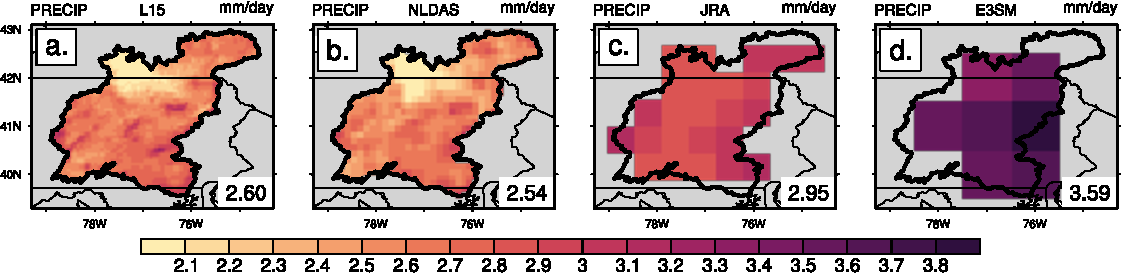
\includegraphics[width=0.98\linewidth]{{figs/cropped/climo_comp_panel_PRECIP}.pdf} \\
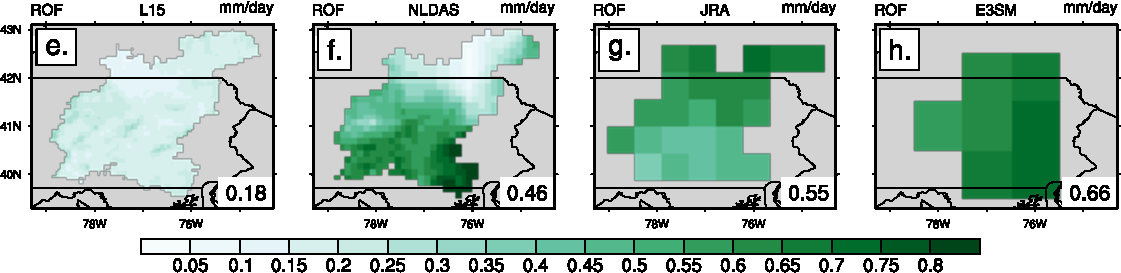
\includegraphics[width=0.98\linewidth]{{figs/cropped/climo_comp_panel_ROF}.pdf} \\
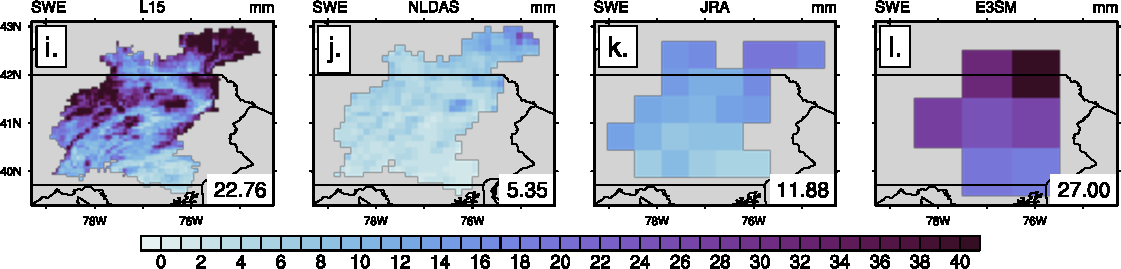
\includegraphics[width=0.98\linewidth]{{figs/cropped/climo_comp_panel_SWE}.pdf} \\
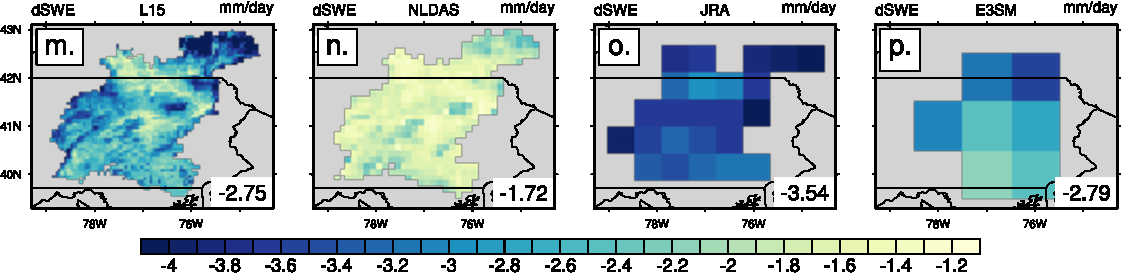
\includegraphics[width=0.98\linewidth]{{figs/cropped/climo_comp_panel_dSWE}.pdf}
\end{tabular}
\caption{November to April mean climatologies of L15, NLDAS, JRA, and E3SM (left to right). From top to bottom are precipitation (PRECIP; mm/day), surface runoff (ROF; mm/day), snow water equivalent (SWE; mm), and daily change in snow water equivalent (dSWE; mm/day). dSWE only includes days with snow loss at a particular grid cell. Data is only included if $>$50\% of a gridded climate data product's cell lies within the SRB bounds (black outline).}
\label{fig:means}
\end{figure}

\begin{table}
\resizebox{\textwidth}{!}{%
\begin{tabular}{lllllllllll}
                & ROF\_t & dSWE\_t & Events & Duration & dSWE & dSWE\_max & ROF & ROF\_max & PRECIP & PRECIP\_max \\
\shortstack{$FIXED$ \\ $(absolute$ $magnitude)$}          &        &         &        &          &      &           &     &          &        &             \\
L15             & 1.4   & 1.4    & 6      & 3.2      & 6.8  & 7.5       & 1.6 & 1.7      & 8.6    & 9.1         \\
NLDAS           & 1.4   & 1.4    & 17     & 3.0      & 3.8  & 4.5       & 1.9 & 2.0      & 5.8    & 6.4         \\
JRA             & 1.4   & 1.4    & 48     & 3.5      & 3.5  & 4.7       & 2.5 & 2.8      & 5.3    & 6.1         \\
E3SM            & 1.4   & 1.4    & 60     & 4.6      & 5.2  & 6.8       & 2.2 & 2.6      & 5.8    & 7.1        \\
                &        &         &        &          &      &           &     &          &        &             \\
\shortstack{$RELATIVE$ \\ $(95th$ $percentile)$} &        &         &        &          &      &           &     &          &        &             \\
L15             & 0.6   & 1.5    & 20     & 6.0      & 4.8  & 6.1       & 0.9 & 1.1      & 5.4    & 6.8         \\
NLDAS           & 1.4   & 0.8    & 21     & 2.9      & 3.2  & 3.8       & 1.9 & 2.0      & 6.1    & 6.7         \\
JRA             & 1.6   & 1.9    & 40     & 3.2      & 4.0  & 5.1       & 2.6 & 2.9      & 5.4    & 6.1         \\
E3SM            & 1.8   & 2.2    & 42     & 4.6      & 6.9  & 8.5       & 2.6 & 3.0      & 6.1    & 7.3          
\end{tabular}
}
\caption{Statistics of rain-on-snow (RoS) flagged events over the SRB (SRB) for several gridded climate data products using FIXED thresholds (top) and RELATIVE thresholds (bottom). Surface runoff (ROF$_t$) and change in daily snow water equivalent (dSWE$_t$) represent the thresholds used. Events represent the number of RoS events flagged over the 1980-2005 period. Duration is the average number of consecutive days an RoS event lasts. dSWE, ROF, and total precipitation (PRECIP) represent the average snow loss, amount of runoff rate, and amount of precipitation rate per event by calculating the mean values across an event and then averaging those. The same variables with a subscript `max' compute the single-day maximum during a given RoS event and represent an average across all the maximas identified.}
\label{table:means}
\end{table}

The differences across gridded climate data products are also shown in Fig. \ref{fig:histograms}. 
All plot subpanels show statistics using RELATIVE, although the same figures for FIXED are shown in the Supplementary Material. 
Figure \ref{fig:histograms}a shows the total number of RoS events flagged over the climatological period (third column of Table \ref{table:means}), while Figures \ref{fig:histograms}b-d show the binned probabilities of daily maximum, basin-averaged, event-level PRECIP, ROF, and dSWE. 
The maximum PRECIP associated with flagged RoS events is similar between the four gridded climate data products, with E3SM tending to have slightly more extreme PRECIP occurring over the SRB (in agreement with Figure \ref{fig:means}). 
Larger differences are seen in ROF and dSWE. 
In ROF, both the E3SM and JRA datasets produce larger event magnitudes of ROF, and subsequently have longer tails in their probability distributions, compared to the other two datasets. 
L15 produces RoS events with the least ROF (averaging approximately one-third of those found in either E3SM or JRA), with NLDAS in between the other three. 
The probability distribution functions of dSWE highlights an even more complex picture, with both NLDAS and L15 having narrower distributions with smaller magnitudes. 
Of note, JRA and E3SM have broader distributions (i.e., longer tails) but the JRA distribution is more skewed, with frequent low dSWE events whereas E3SM has a more uniform distribution of dSWE rates.

In summary, using either a relative or fixed threshold to identify RoS events, the fully-coupled ESMs (E3SM and JRA) produce more events than L15 and NLDAS.
While daily PRECIP in each product differs somewhat, it should be noted that these differences are relatively small.
Rather, the majority of the differences in RoS events flagged arise from lower magnitudes of ROF (dSWE) in the L15 (NLDAS). 
It is worth noting that L15 and NLDAS produce fewer RoS events regardless of which thresholding is used, so not only are the distributions of relevant daily variables shifted relative to the other models, but their skewness is impacted as well (Fig. \ref{fig:histograms}).

\begin{figure}
\begin{tabular}{cc}
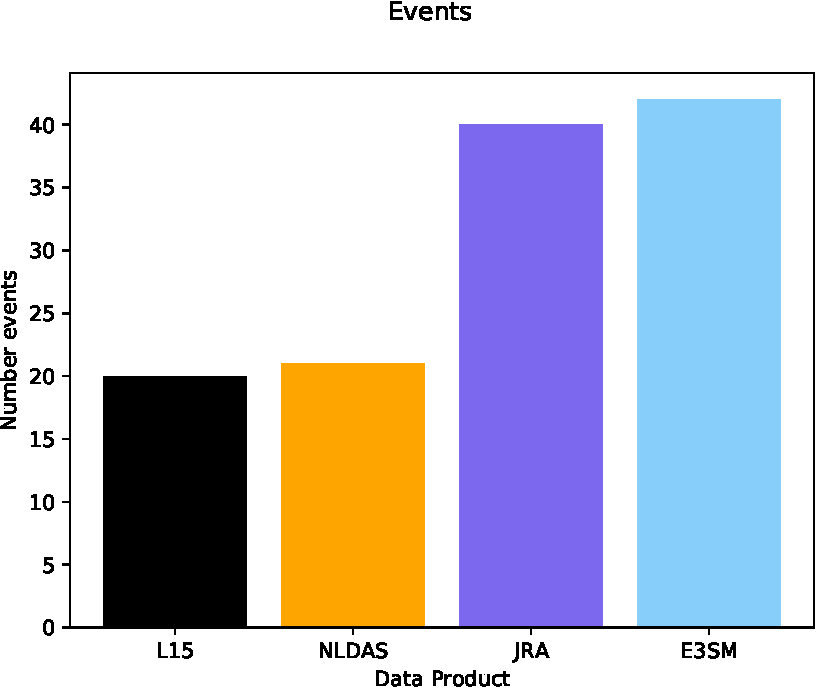
\includegraphics[width=0.442\linewidth]{{figs/cropped/events_95}.pdf} & 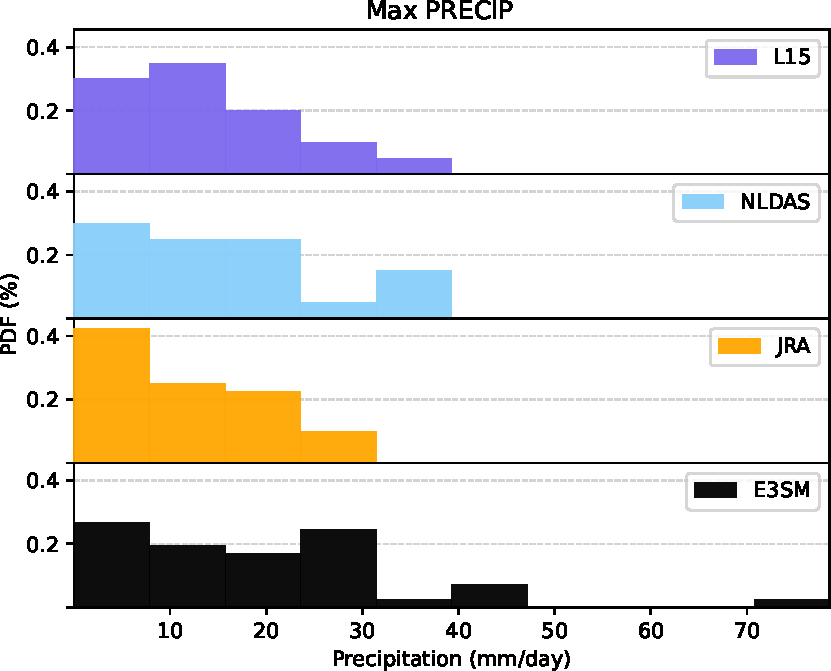
\includegraphics[width=0.451\linewidth]{{figs/cropped/Max_precip_95}.pdf} \\
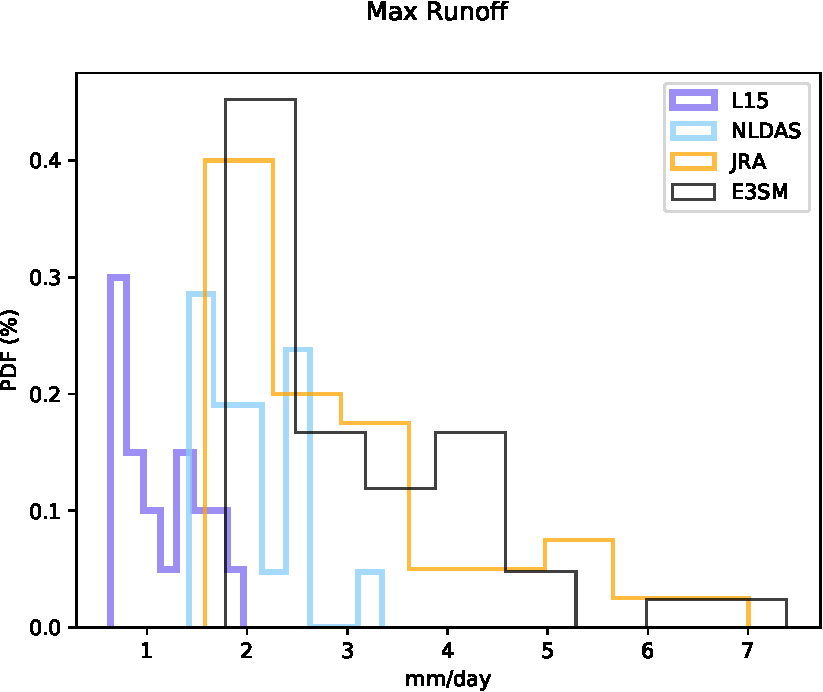
\includegraphics[width=0.451\linewidth]{{figs/cropped/Max_runoff_95}.pdf} & 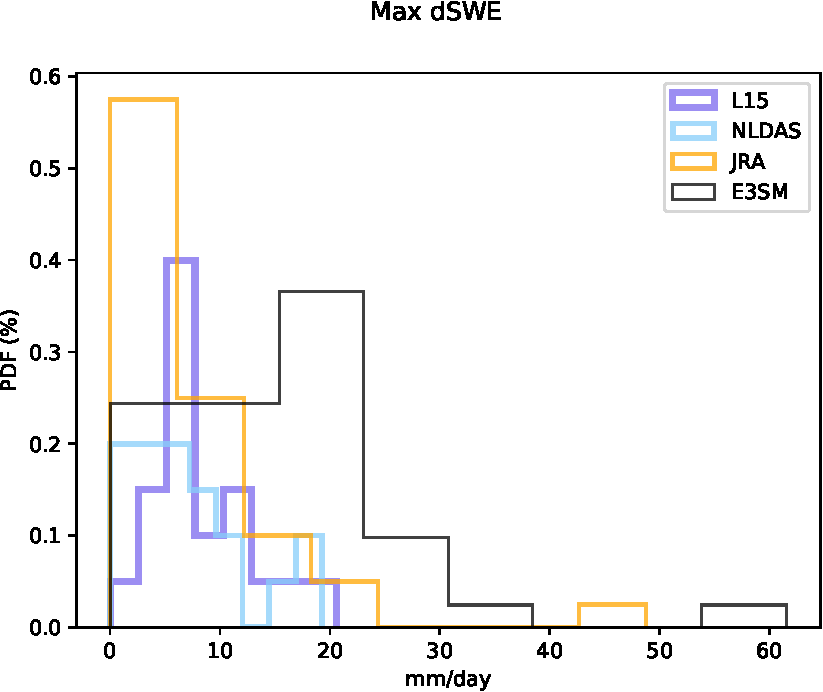
\includegraphics[width=0.451\linewidth]{{figs/cropped/Max_dSWE_95}.pdf}
\end{tabular}
\caption{Histogram statistics for RoS events across the data products for the RELATIVE detection framework. The number of RoS events for each product from 1985-2005 is shown in the top left. In the other three panels, frequency distributions of the rate (mm/day) of maximum precipitation (PRECIP), maximum runoff (ROF), and maximum daily change in snow water equivalent (dSWE) for each flagged RoS event are shown.}
\label{fig:histograms}
\end{figure}

\subsection{Single-year evaluation}

%\begin{figure}
%\begin{tabular}{cc}
%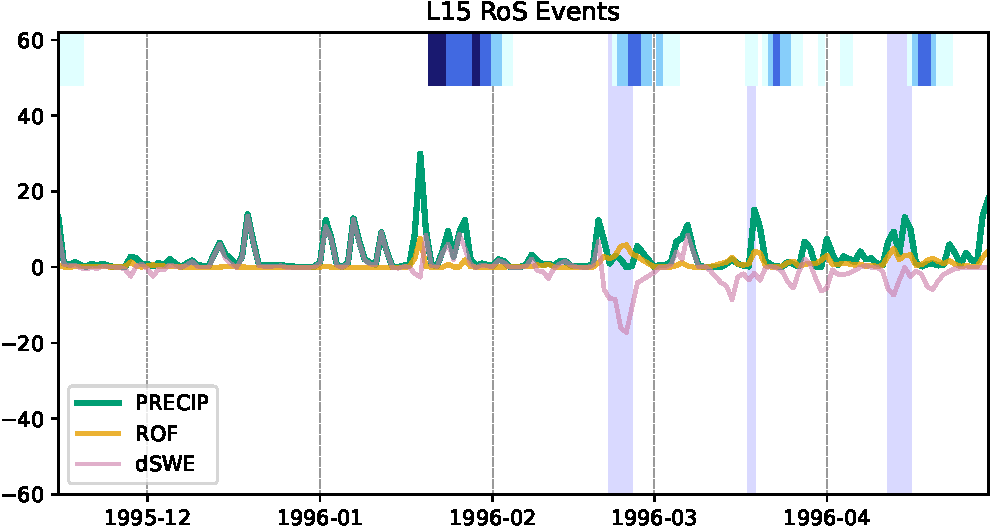
\includegraphics[width=0.45\linewidth]{{figs/cropped/L15_1995_events}.pdf} & 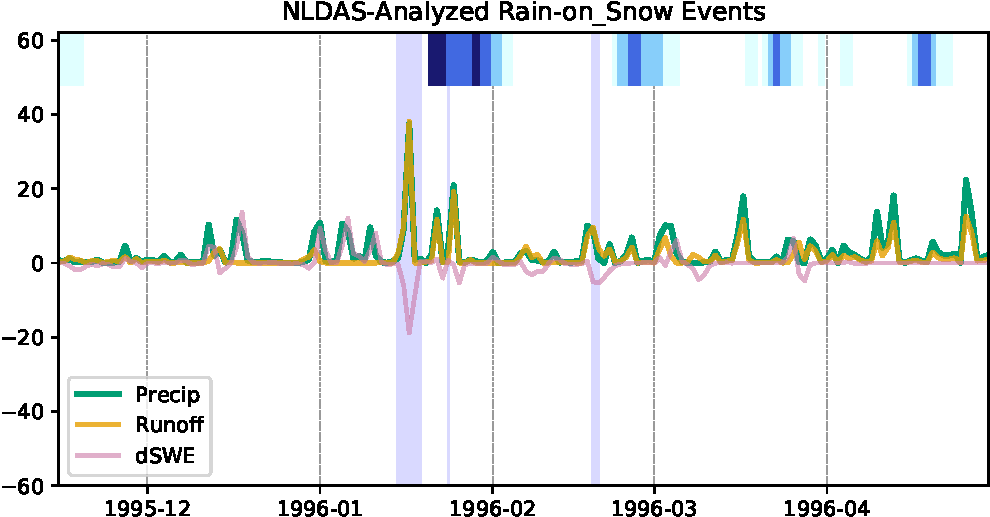
\includegraphics[width=0.45\linewidth]{{figs/cropped/NLDAS_1995_events}.pdf} \\
%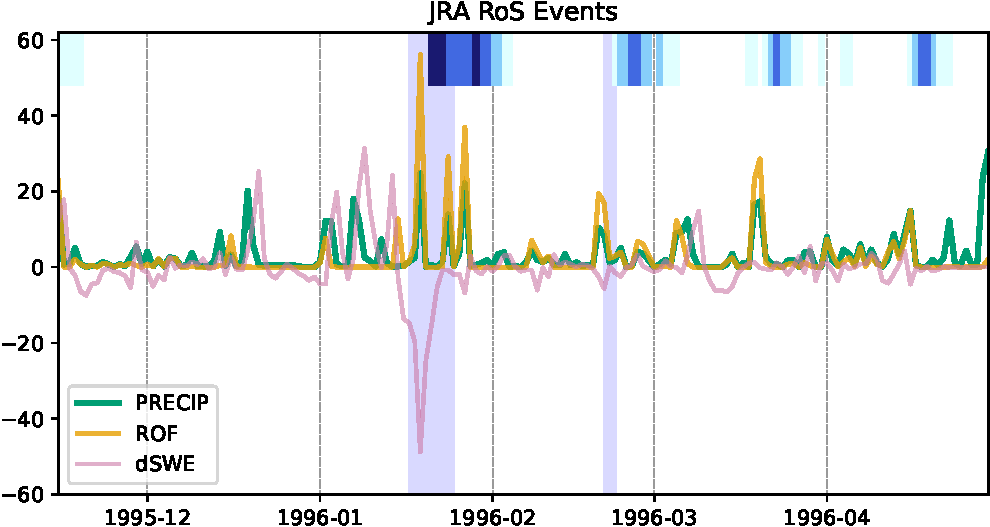
\includegraphics[width=0.45\linewidth]{{figs/cropped/JRA_1995_events}.pdf} & 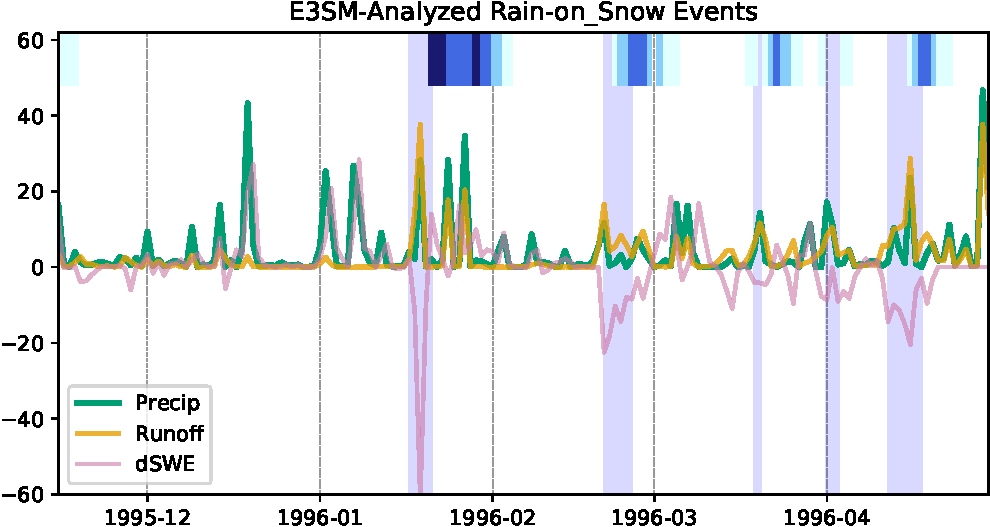
\includegraphics[width=0.45\linewidth]{{figs/cropped/E3SM_1995_events}.pdf}
%\end{tabular}
%\caption{Timeseries of daily precipitation (green), surface runoff (orange), and snow loss (pink) during WY95 for each of the four products. Vertical purple shading denotes periods flagged as a rain-on-snow event by the method discussed in methods. At the top of each timeseries is a colored bar series which denotes extreme values (greater than 75\%) of observed USGS streamflow at Harrisburg, with very dark hues representing 99\% values over the 1980-2005 period.}
%\label{fig:yr-timeseries-comp}
%\end{figure}
%
%\begin{figure}
%\begin{tabular}{cc}
%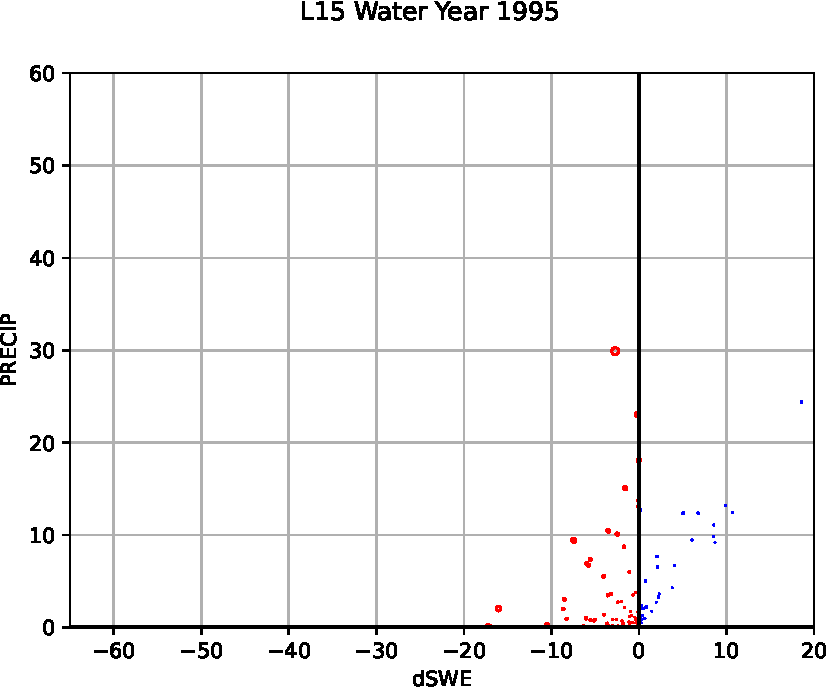
\includegraphics[width=0.45\linewidth]{{figs/cropped/L15_1995_scatplot}.pdf} & 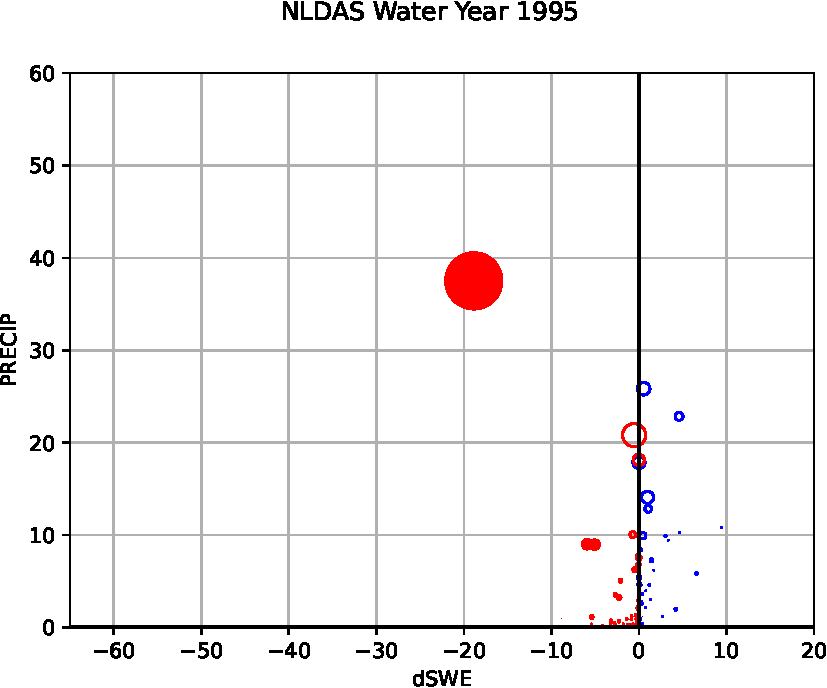
\includegraphics[width=0.45\linewidth]{{figs/cropped/NLDAS_1995_scatplot}.pdf} \\
%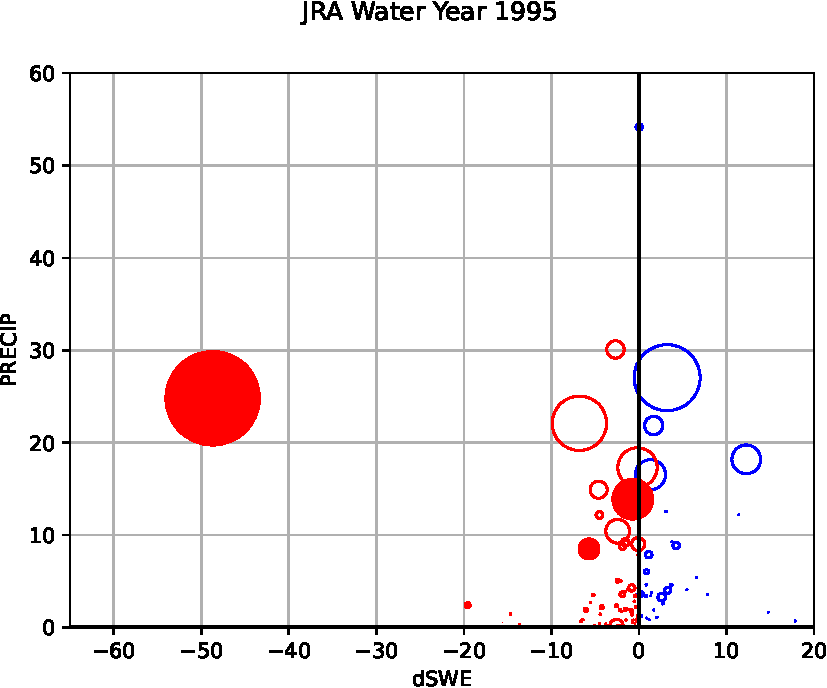
\includegraphics[width=0.45\linewidth]{{figs/cropped/JRA_1995_scatplot}.pdf} & 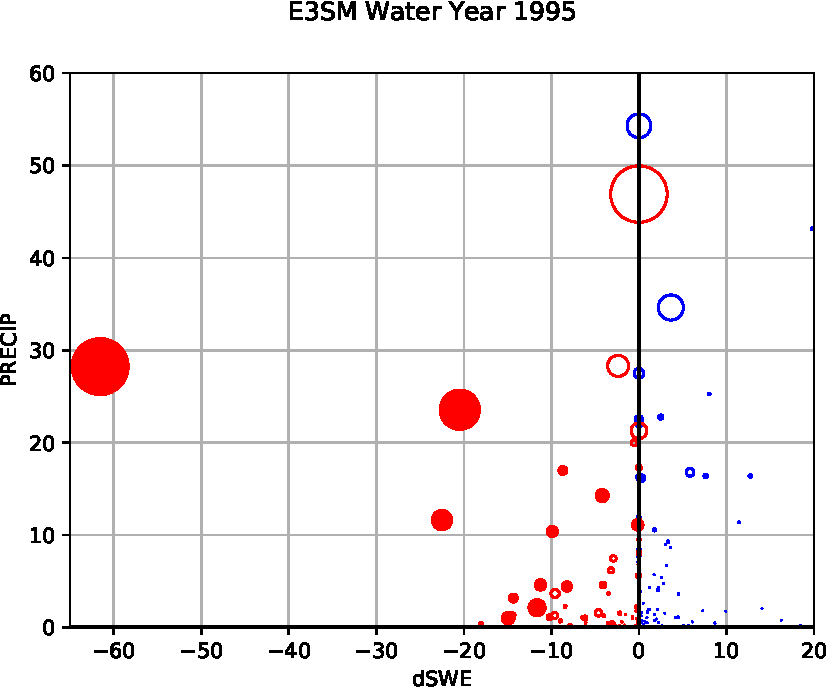
\includegraphics[width=0.45\linewidth]{{figs/cropped/E3SM_1995_scatplot}.pdf}
%\end{tabular}
%\caption{Bubble plots comparing precipitation (y-axis), SWE change (x-axis), and surface runoff (size of bubble) for each of the four datasets during WY95. For each bubble, the values used come from the same calendar day. Bubbles that are filled were flagged by the algorithm as a rain-on-snow event (purple shaded periods in Fig. \ref{yr-timeseries-comp}).}
%\label{fig:bubble-comp}
%\end{figure}

\begin{figure}
\centering
\begin{tabularx}{\textwidth}{XX}
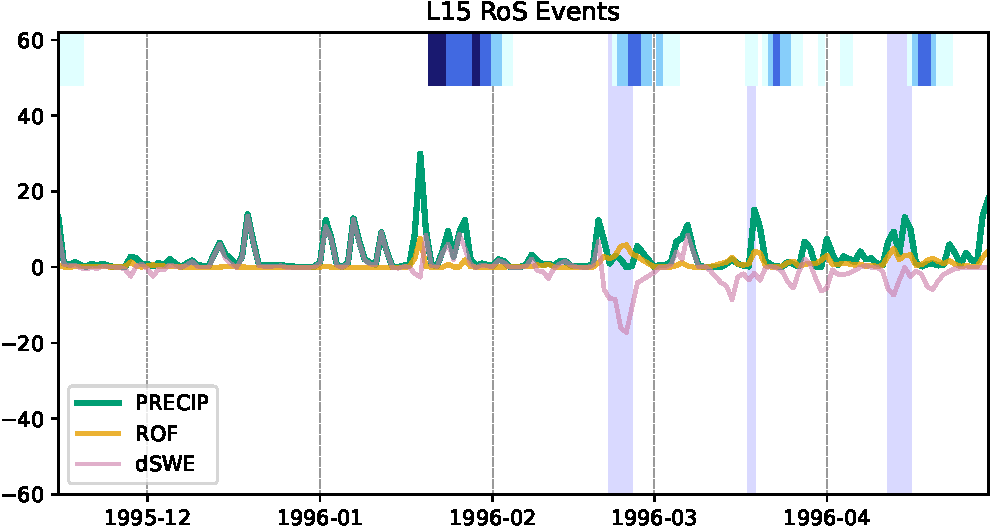
\includegraphics[width=1.0\linewidth]{{figs/cropped/L15_1995_events}.pdf} & 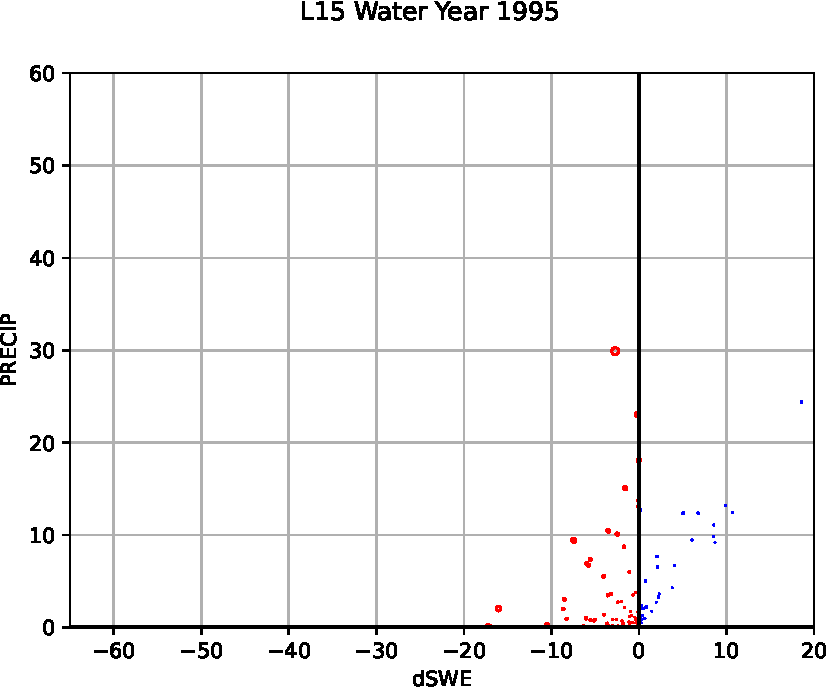
\includegraphics[width=0.75\linewidth]{{figs/cropped/L15_1995_scatplot}.pdf} \\ 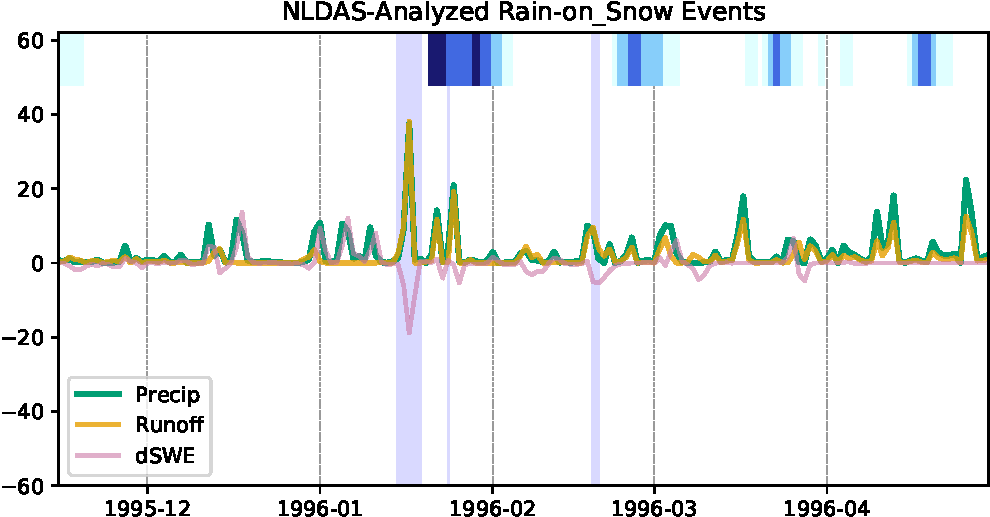
\includegraphics[width=1.0\linewidth]{{figs/cropped/NLDAS_1995_events}.pdf} & 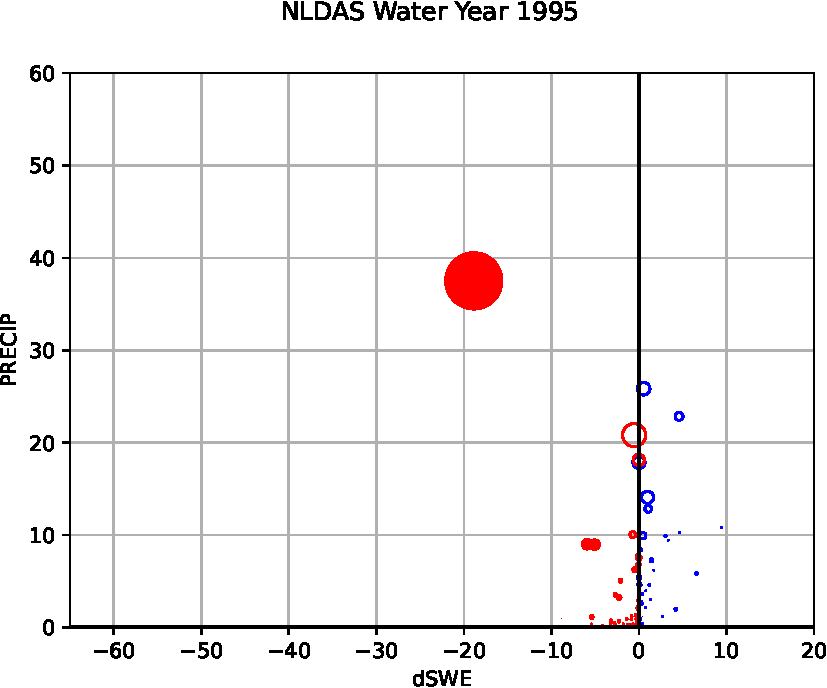
\includegraphics[width=0.75\linewidth]{{figs/cropped/NLDAS_1995_scatplot}.pdf} \\
    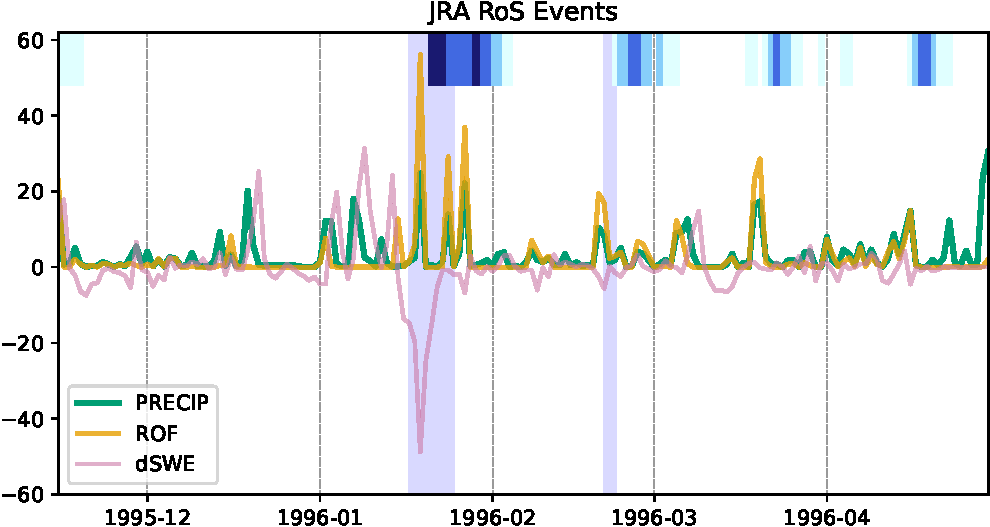
\includegraphics[width=1.0\linewidth]{{figs/cropped/JRA_1995_events}.pdf} & 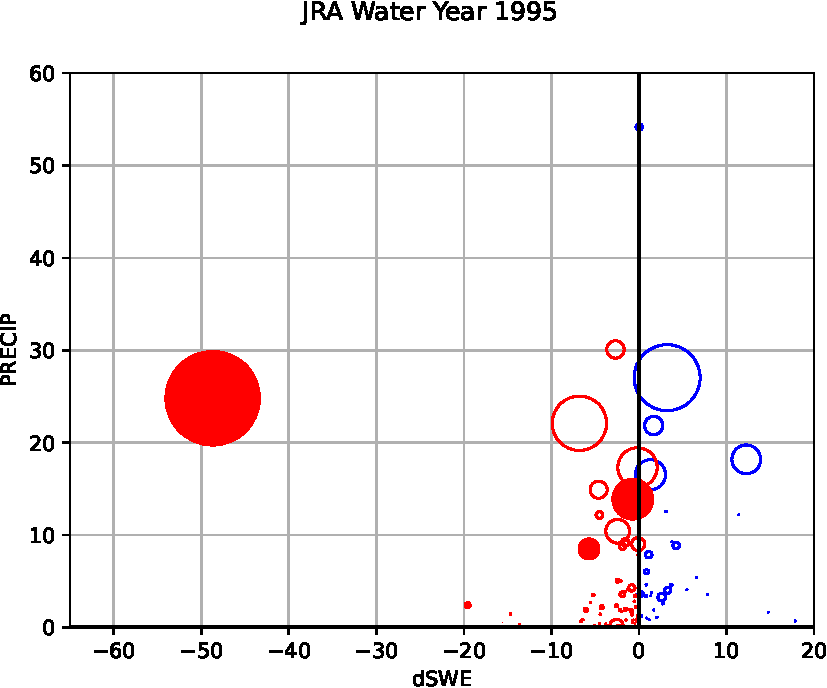
\includegraphics[width=0.75\linewidth]{{figs/cropped/JRA_1995_scatplot}.pdf} \\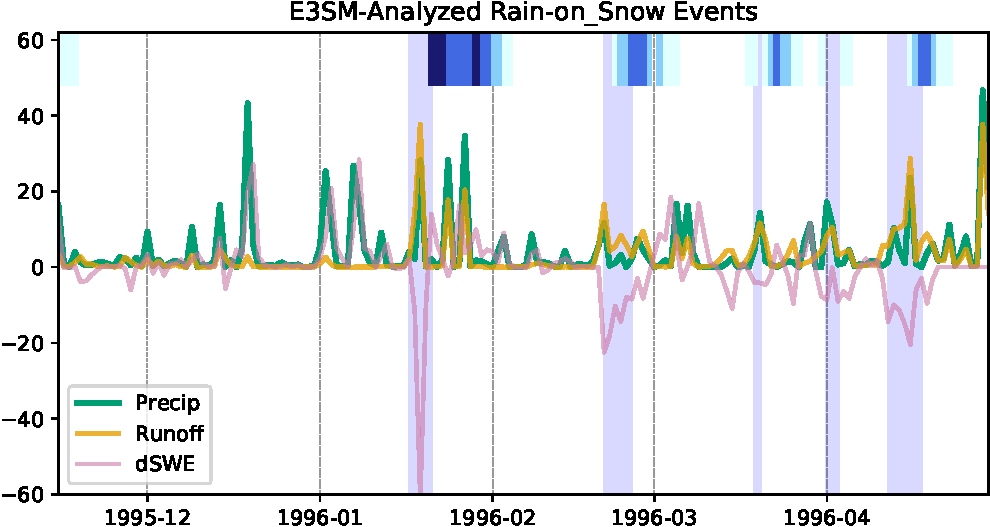
\includegraphics[width=1.0\linewidth]{{figs/cropped/E3SM_1995_events}.pdf} & 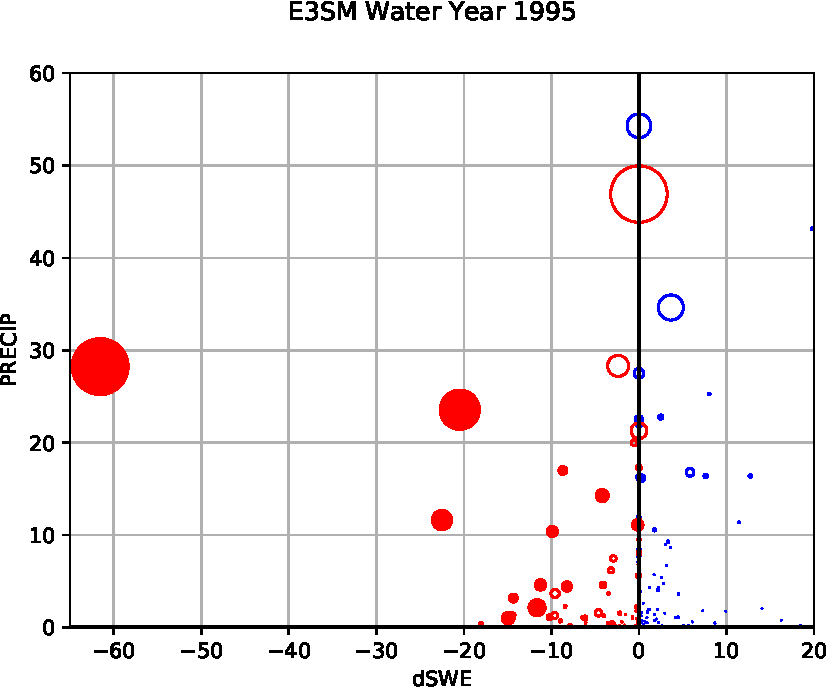
\includegraphics[width=0.75\linewidth]{{figs/cropped/E3SM_1995_scatplot}.pdf}
\end{tabularx}
\caption{(left) Time series of daily precipitation (PRECIP; green), surface runoff (ROF; orange), and change in snow water equivalent (dSWE; pink) during WY95 for each of the four gridded climate data products. Vertical purple shading denotes periods flagged as a rain-on-snow (RoS) event using frameworks discussed in the Methods. Along the top x-axis of each time series is a colored bar series which denotes extreme values (greater than 75\%) of observed USGS streamflow at Harrisburg, PA with the darkest hues representing 99\% values over the 1980-2005 period. (right) Bubble plots comparing PRECIP (y-axis), dSWE (x-axis), and ROF (size of bubble) for each of the four gridded climate data products during WY95. For each bubble, the values used are derived from the same calendar day. Bubbles that are filled were flagged by the RoS algorithm as an RoS event.}
\label{fig:merged-wy}
\end{figure}

To further explore RoS events at the singular feature level we focus on results associated with the 1995 water year (WY95, October 1995 to September 1996). We choose this WY since this includes the 1996 SRB flood that is often used in water management circles for disaster planning purposes \citep{leathers1998severe}. 
The same visualizations for other WYs are shown in the Supplemental Material.

Figure \ref{fig:merged-wy} (left) shows the daily WY95 time series of basin-integrated PRECIP, ROF, and dSWE.
Negative (positive) dSWE denotes snowmelt (accumulation). 
Vertical shading denotes RoS events that were flagged by the algorithm. 
At the top of each panel is a stripe with four different gradient shadings, representing days where streamflow exceeded 75\%, 90\%, 95\%, and 99\% relative over the 1985-2005 period at the US Geological Survey (USGS) gauge at Harrisburg, Pennsylvania (USGS \#01570500), with darker colors representing anomalously high flow conditions.

The January 17-18, 1996 event is readily apparent for three of the four data products (NLDAS, JRA, E3SM). 
Observed streamflow spiked during and immediately after the RoS event as shown by the dark blue stripes at the top of each time series, indicating a lag between when the RoS event algorithm identifies changes in PRECIP, dSWE, and ROF across the gridded climate data products and the observed daily streamflow gauge observation at Harrisburg, PA (namely, the 99th percentile streamflow exceedance).
While this is operationally the largest RoS event observed over the period, there remains large discrepancies between the datasets. 
The dSWE signal is largest in magnitude within JRA and E3SM compared to NLDAS. 
L15 shows a very minimal dSWE, to the point that the RoS event thresholds are not triggered in the detection algorithm. 
PRECIP is more similar across the three datasets, implying that the reduced ROF in L15 is likely due to the lack of snowmelt.

All products also indicate a second, more moderate RoS event during the last third of February, although L15 and E3SM (JRA and E3SM) show larger dSWE (ROF) signals than the other two datasets. 
The USGS streamflow also exceeded the 95th percentile for this RoS event. 
More moderate flooding also appeared to occur in March and April although the detection algorithm only flagged an event in L15 and E3SM. 
Given that all RoS events flagged by the detection algorithm result in well-above-average streamflow highlights the efficacy of the detection algorithm in capturing meaningful hydrometeorological extremes.

Another way to visualize the WY95 RoS events is shown in Figure \ref{fig:merged-wy} (right).  This plot shows the daily distribution of all three quantities by plotting dSWE on the x-axis, PRECIP on the y-axis, and the size of the x-y marker depicts the magnitude of ROF.
Markers are filled if the RoS event criteria is triggered for that calendar day and are colored red (blue) if there is dSWE loss (gain). 
The variability of the PRECIP (y-axis) is the most similar between the two ESMs.
The vast majority of daily basin-scale precipitation remains below 30 mm/day, although E3SM produces a few days with more extreme precipitation rates (which agrees with E3SM being a slightly ``wetter'' product). 
Larger differences across datasets are noted for the other two RoS event response variables. 
JRA and E3SM produce a wide spread in both RoS and non-RoS events along the y-axis, indicating that the fully-coupled ESMs produce days with the largest magnitudes of dSWE. 
Further, L15 has markers that are small in size, indicating low daily ROF magnitudes when compared to the other three products.
There is a substantial spread across the four datasets, even over comparable time series with well-defined and record-setting RoS events.
This is likely due to daily differences in the timing of storms, the amount of precipitation they produce, and how close surface air temperatures are to freezing conditions that in turn influence if a meteorological event leads to an increase in snow accumulation or results in an RoS event.

\section{Discussion}

We interrogate four different gridded climate data products, that include PRECIP, ROF, and SWE, in order to quantify differences in the representation of coupled land-atmosphere processes that lead to flooding events in the historical record.
In particular, we focus on RoS floods over the SRB and devise an algorithm for automatic detection of these events that can be applied across any desired dataset. 

Detection algorithm flagging for times of collocated ROF and dSWE does a reasonable job of marking periods that will be followed by above-normal streamflow. 
We find using fixed thresholds for RoS-relevant variables applied uniformly across multiple gridded datasets leads to large discrepancies in event frequency over the historical period, up to a factor of 10. 
Normalizing these thresholds by each datasets' climatology (relative thresholds based on daily percentiles) improves agreement. 
However, there remains approximately a factor of two difference between event counts, implying that the underlying distributions are fundamentally different in both shape and magnitude across the data analyzed.

% Notably, although we refer to automated algorithm-flagged events as RoS events, there is no explicit PRECIP threshold. 
% With that said, we find that 75\% of automated algorithm-flagged events have at least one day of $>5$ mm/day of basin-averaged precipitation and 95\% have at least one day of measurable precipitation ($>$1 mm/day).
% This implies that while ablation-only snowmelt events can lead to flooding, the vast majority of events producing large flood signals involve some form of precipitation as well.

This underscores the complex assessment of such flood events. 
%A common misconception is that RoS events are generated by warm rain transferring heat to the snowpack which then ripens or ablates it. 
Multiple studies have found that the actual heat transfer between the liquid rain and surface snowpack is rather small and explains only a small fraction of the observed snowmelt \citep{moore1984controls}. 
Rather, factors such as surface humidity and temperature (and associated latent and sensible heat fluxes) and downwelling radiation into the snowpack are more dominant drivers of snow ablation \citep{mazurkiewicz2008assessing,wurzer2016influence,harpold2018humidity}. 
It is evident that similar synoptic meteorological patterns \citep{grote2021synoptic} and additional liquid input to the surface (i.e., runoff being a combination of snowmelt and water flux from the atmosphere) leads to the majority of RoS events being associated with at least some precipitation.

The spatiotemporal dependencies of how meteorological data is generated for land surface and/or hydrological model forcing are critically important. 
While spatial resolution of data is important, particularly for snow processes in complex terrain \citep{henn2018an,Woodburn2021}, we show that the time resolution of data is just as critical for transient extremes, such as RoS events.
This is because the timing of synoptic variations in surface temperature and humidity that dictate snowmelt and precipitation phase can occur on the order of hours at local scales and can have an outsized role in compound extreme event representation if those variations are threshold-dependent (e.g., storm rain-snow partitioning and alterations to the freezing line at the land surface).
Since RoS events in regions of ephemeral snow (e.g., SRB) can have rapid changes in surface forcing at hourly timescales (e.g., \citet{leathers1998severe}), using daily meteorological data (as in NLDAS and L15) to force offline land surface models may result in an underprediction of RoS frequency. 
This may occur if time-interpolated data (and less frequent coupling) clips short-term extrema and results in mismatched forcing or reduced day-to-day variability of multiple, co-dependent anomalies (e.g., temperature and precipitation extremes) required to accurately simulate historical, decision-relevant hydrometeorological extremes (e.g., 1996 SRB RoS event). 
We show that even though a dataset is provided at much coarser spatial resolutions than is desired (e.g., JRA), model-derived datasets that are more frequently coupled and/or constrained at shorter timescales (e.g., reanalysis products and nudged ESMs) produce more accurate land-atmosphere interactions and better representation of decision-relevant hydrometeorological extremes. 
It is recommended that gridded climate data product developers consider the temporal resolution of land surface forcing if the representation of such daily hydrometeorological extrema is desirable, particularly from a use-inspired or decision-relevant context \citep{Jagannathan2021}.
While we do not downscale any datasets in this study, it is likely that using different meteorological data to force the same land surface and/or hydrological model will result in vastly different predicted streamflows, particularly for RoS events when variables are spatiotemporally co-dependent and would be sensitive to any post-processing adjustments in the gridded climate data product (e.g., mean climatological correction). 

From a stakeholder perspective, this is an important consideration when back-testing models, and, in particular, applying such models to evaluate tail risks (e.g., 1-in-100 year flood events and how they may change in a future climate). 
The results here show longer tails in the fully-coupled ESM-derived gridded climate data, which may impact return rates of hydrometeorological extreme events, even if calibrated. 
Therefore, care must be taken when applying data requiring coupling between the atmosphere and land surface (and riverine) components, whether generated dynamically or statistically. 
While post-processing adjustments to the mean climatology may be desirable, these adjustments can alter decision-relevant hydrometeorological events that reside in the tail of the distribution.



%%

%  Numbered lines in equations:
%  To add line numbers to lines in equations,
%  \begin{linenomath*}
%  \begin{equation}
%  \end{equation}
%  \end{linenomath*}



%% Enter Figures and Tables near as possible to where they are first mentioned:
%
% DO NOT USE \psfrag or \subfigure commands.
%
% Figure captions go below the figure.
% Table titles go above tables;  other caption information
%  should be placed in last line of the table, using
% \multicolumn2l{$^a$ This is a table note.}
%
%----------------
% EXAMPLE FIGURES
%
% \begin{figure}
% \includegraphics{example.png}
% \caption{caption}
% \end{figure}
%
% Giving latex a width will help it to scale the figure properly. A simple trick is to use \textwidth. Try this if large figures run off the side of the page.
% \begin{figure}
% \noindent\includegraphics[width=\textwidth]{anothersample.png}
%\caption{caption}
%\label{pngfiguresample}
%\end{figure}
%
%
% If you get an error about an unknown bounding box, try specifying the width and height of the figure with the natwidth and natheight options. This is common when trying to add a PDF figure without pdflatex.
% \begin{figure}
% \noindent\includegraphics[natwidth=800px,natheight=600px]{samplefigure.pdf}
%\caption{caption}
%\label{pdffiguresample}
%\end{figure}
%
%
% PDFLatex does not seem to be able to process EPS figures. You may want to try the epstopdf package.
%

%
% ---------------
% EXAMPLE TABLE
%
% \begin{table}
% \caption{Time of the Transition Between Phase 1 and Phase 2$^{a}$}
% \centering
% \begin{tabular}{l c}
% \hline
%  Run  & Time (min)  \\
% \hline
%   $l1$  & 260   \\
%   $l2$  & 300   \\
%   $l3$  & 340   \\
%   $h1$  & 270   \\
%   $h2$  & 250   \\
%   $h3$  & 380   \\
%   $r1$  & 370   \\
%   $r2$  & 390   \\
% \hline
% \multicolumn{2}{l}{$^{a}$Footnote text here.}
% \end{tabular}
% \end{table}

%% SIDEWAYS FIGURE and TABLE
% AGU prefers the use of {sidewaystable} over {landscapetable} as it causes fewer problems.
%
% \begin{sidewaysfigure}
% \includegraphics[width=20pc]{figsamp}
% \caption{caption here}
% \label{newfig}
% \end{sidewaysfigure}
%
%  \begin{sidewaystable}
%  \caption{Caption here}
% \label{tab:signif_gap_clos}
%  \begin{tabular}{ccc}
% one&two&three\\
% four&five&six
%  \end{tabular}
%  \end{sidewaystable}

%% If using numbered lines, please surround equations with \begin{linenomath*}...\end{linenomath*}
%\begin{linenomath*}
%\begin{equation}
%y|{f} \sim g(m, \sigma),
%\end{equation}
%\end{linenomath*}

%%% End of body of article

%%%%%%%%%%%%%%%%%%%%%%%%%%%%%%%%
%% Optional Appendix goes here
%
% The \appendix command resets counters and redefines section heads
%
% After typing \appendix
%
%\section{Here Is Appendix Title}
% will show
% A: Here Is Appendix Title
%
%\appendix
%\section{Here is a sample appendix}

%%%%%%%%%%%%%%%%%%%%%%%%%%%%%%%%%%%%%%%%%%%%%%%%%%%%%%%%%%%%%%%%
%
% Optional Glossary, Notation or Acronym section goes here:
%
%%%%%%%%%%%%%%
% Glossary is only allowed in Reviews of Geophysics
%  \begin{glossary}
%  \term{Term}
%   Term Definition here
%  \term{Term}
%   Term Definition here
%  \term{Term}
%   Term Definition here
%  \end{glossary}

%
%%%%%%%%%%%%%%
% Acronyms
%   \begin{acronyms}
%   \acro{Acronym}
%   Definition here
%   \acro{EMOS}
%   Ensemble model output statistics
%   \acro{ECMWF}
%   Centre for Medium-Range Weather Forecasts
%   \end{acronyms}

%
%%%%%%%%%%%%%%
% Notation
%   \begin{notation}
%   \notation{$a+b$} Notation Definition here
%   \notation{$e=mc^2$}
%   Equation in German-born physicist Albert Einstein's theory of special
%  relativity that showed that the increased relativistic mass ($m$) of a
%  body comes from the energy of motion of the body—that is, its kinetic
%  energy ($E$)—divided by the speed of light squared ($c^2$).
%   \end{notation}


\section{Open Research}

The SRB is defined using a shapefile provided by the SRB Commission (\url{https://www.srbc.net/portals/susquehanna-atlas/data-and-maps/subbasins/index.html}). L15 data was downloaded from the National Oceanic and Atmospheric Administration Physical Science Laboratory, available at \url{https://psl.noaa.gov/data/gridded/data.livneh.html}. NLDAS-VIC data was downloaded from NCEP, available at \url{ftp://ldas.ncep.noaa.gov/nldas2/retrospective/vic4.0.5}. JRA-55 data was downloaded from the Research Data Archive at the National Center for Atmospheric Research, Computational and Information Systems Laboratory, available at \url{https://doi.org/10.5065/D6HH6H41}. The version of E3SM run here was v2.0.0-alpha.2-1816-gf9cbe57a2 and is available at https://github.com/E3SM-Project/E3SM. ERA5 data used to nudge the E3SM solution was downloaded from the Copernicus Climate Data Store (CDS), available at \url{https://www.ecmwf.int/en/forecasts/datasets/reanalysis-datasets/era5}. All data and scripts used to generate the figures contained in this manuscript are currently available at \url{xxxxxx} and will be uploaded to Zenodo, given a DOI, and linked [here] upon acceptance.



%%%%%%%%%%%%%%%%%%%%%%%%%%%%%%%%%%%%%%%%%%%%%%%%%%%%%%%%%%%%%%%%
%
%  ACKNOWLEDGMENTS
%
% The acknowledgments must list:
%
% >>>>	A statement that indicates to the reader where the data
% 	supporting the conclusions can be obtained (for example, in the
% 	references, tables, supporting information, and other databases).
%
% 	All funding sources related to this work from all authors
%
% 	Any real or perceived financial conflicts of interests for any
%	author
%
% 	Other affiliations for any author that may be perceived as
% 	having a conflict of interest with respect to the results of this
% 	paper.
%
%
% It is also the appropriate place to thank colleagues and other contributors.
% AGU does not normally allow dedications.


\acknowledgments
This work is supported by the U.S. Department of Energy (DOE), Office of Science, Office of Biological and Environmental Research program under Award DE-SC0016605 ``A framework for improving analysis and modeling of Earth system and intersectoral dynamics at regional scales.'' Data acquisition and E3SM simulations were completed at the DOE National Energy Research Scientific Computing Center (NERSC) at Lawrence Berkeley National Laboratory (DE-AC02-05CH11231) using NERSC award ERCAP0020801. Event algorithm development, calibration, and analysis was performed on the Pennsylvania State University's Institute for Computational and Data Sciences' Roar supercomputer.


%% ------------------------------------------------------------------------ %%
%% References and Citations

%%%%%%%%%%%%%%%%%%%%%%%%%%%%%%%%%%%%%%%%%%%%%%%
%
% \bibliography{<name of your .bib file>} don't specify the file extension
%
% don't specify bibliographystyle
%%%%%%%%%%%%%%%%%%%%%%%%%%%%%%%%%%%%%%%%%%%%%%%

\bibliography{refs-ros-metrics}

%Reference citation instructions and examples:
%
% Please use ONLY \cite and \citeA for reference citations.
% \cite for parenthetical references
% ...as shown in recent studies (Simpson et al., 2019)
% \citeA for in-text citations
% ...Simpson et al. (2019) have shown...
%
%
%...as shown by \citeA{jskilby}.
%...as shown by \citeA{lewin76}, \citeA{carson86}, \citeA{bartoldy02}, and \citeA{rinaldi03}.
%...has been shown \cite{jskilbye}.
%...has been shown \cite{lewin76,carson86,bartoldy02,rinaldi03}.
%... \cite <i.e.>[]{lewin76,carson86,bartoldy02,rinaldi03}.
%...has been shown by \cite <e.g.,>[and others]{lewin76}.
%
% apacite uses < > for prenotes and [ ] for postnotes
% DO NOT use other cite commands (e.g., \citet, \citep, \citeyear, \nocite, \citealp, etc.).
%



\end{document}



More Information and Advice:

%% ------------------------------------------------------------------------ %%
%
%  SECTION HEADS
%
%% ------------------------------------------------------------------------ %%

% Capitalize the first letter of each word (except for
% prepositions, conjunctions, and articles that are
% three or fewer letters).

% AGU follows standard outline style; therefore, there cannot be a section 1 without
% a section 2, or a section 2.3.1 without a section 2.3.2.
% Please make sure your section numbers are balanced.
% ---------------
% Level 1 head
%
% Use the \section{} command to identify level 1 heads;
% type the appropriate head wording between the curly
% brackets, as shown below.
%
%An example:
%\section{Level 1 Head: Introduction}
%
% ---------------
% Level 2 head
%
% Use the \subsection{} command to identify level 2 heads.
%An example:
%\subsection{Level 2 Head}
%
% ---------------
% Level 3 head
%
% Use the \subsubsection{} command to identify level 3 heads
%An example:
%\subsubsection{Level 3 Head}
%
%---------------
% Level 4 head
%
% Use the \subsubsubsection{} command to identify level 3 heads
% An example:
%\subsubsubsection{Level 4 Head} An example.
%
%% ------------------------------------------------------------------------ %%
%
%  IN-TEXT LISTS
%
%% ------------------------------------------------------------------------ %%
%
% Do not use bulleted lists; enumerated lists are okay.
% \begin{enumerate}
% \item
% \item
% \item
% \end{enumerate}
%
%% ------------------------------------------------------------------------ %%
%
%  EQUATIONS
%
%% ------------------------------------------------------------------------ %%

% Single-line equations are centered.
% Equation arrays will appear left-aligned.

Math coded inside display math mode \[ ...\]
 will not be numbered, e.g.,:
 \[ x^2=y^2 + z^2\]

 Math coded inside \begin{equation} and \end{equation} will
 be automatically numbered, e.g.,:
 \begin{equation}
 x^2=y^2 + z^2
 \end{equation}


% To create multiline equations, use the
% \begin{eqnarray} and \end{eqnarray} environment
% as demonstrated below.
\begin{eqnarray}
  x_{1} & = & (x - x_{0}) \cos \Theta \nonumber \\
        && + (y - y_{0}) \sin \Theta  \nonumber \\
  y_{1} & = & -(x - x_{0}) \sin \Theta \nonumber \\
        && + (y - y_{0}) \cos \Theta.
\end{eqnarray}

%If you don't want an equation number, use the star form:
%\begin{eqnarray*}...\end{eqnarray*}

% Break each line at a sign of operation
% (+, -, etc.) if possible, with the sign of operation
% on the new line.

% Indent second and subsequent lines to align with
% the first character following the equal sign on the
% first line.

% Use an \hspace{} command to insert horizontal space
% into your equation if necessary. Place an appropriate
% unit of measure between the curly braces, e.g.
% \hspace{1in}; you may have to experiment to achieve
% the correct amount of space.


%% ------------------------------------------------------------------------ %%
%
%  EQUATION NUMBERING: COUNTER
%
%% ------------------------------------------------------------------------ %%

% You may change equation numbering by resetting
% the equation counter or by explicitly numbering
% an equation.

% To explicitly number an equation, type \eqnum{}
% (with the desired number between the brackets)
% after the \begin{equation} or \begin{eqnarray}
% command.  The \eqnum{} command will affect only
% the equation it appears with; LaTeX will number
% any equations appearing later in the manuscript
% according to the equation counter.
%

% If you have a multiline equation that needs only
% one equation number, use a \nonumber command in
% front of the double backslashes (\\) as shown in
% the multiline equation above.

% If you are using line numbers, remember to surround
% equations with \begin{linenomath*}...\end{linenomath*}

%  To add line numbers to lines in equations:
%  \begin{linenomath*}
%  \begin{equation}
%  \end{equation}
%  \end{linenomath*}



